
\subsubsection{Topology Optimization} \label{sec:topology optimization}
\begin{figure*}
	\centering
	\begin{subfigure}{1\textwidth}
		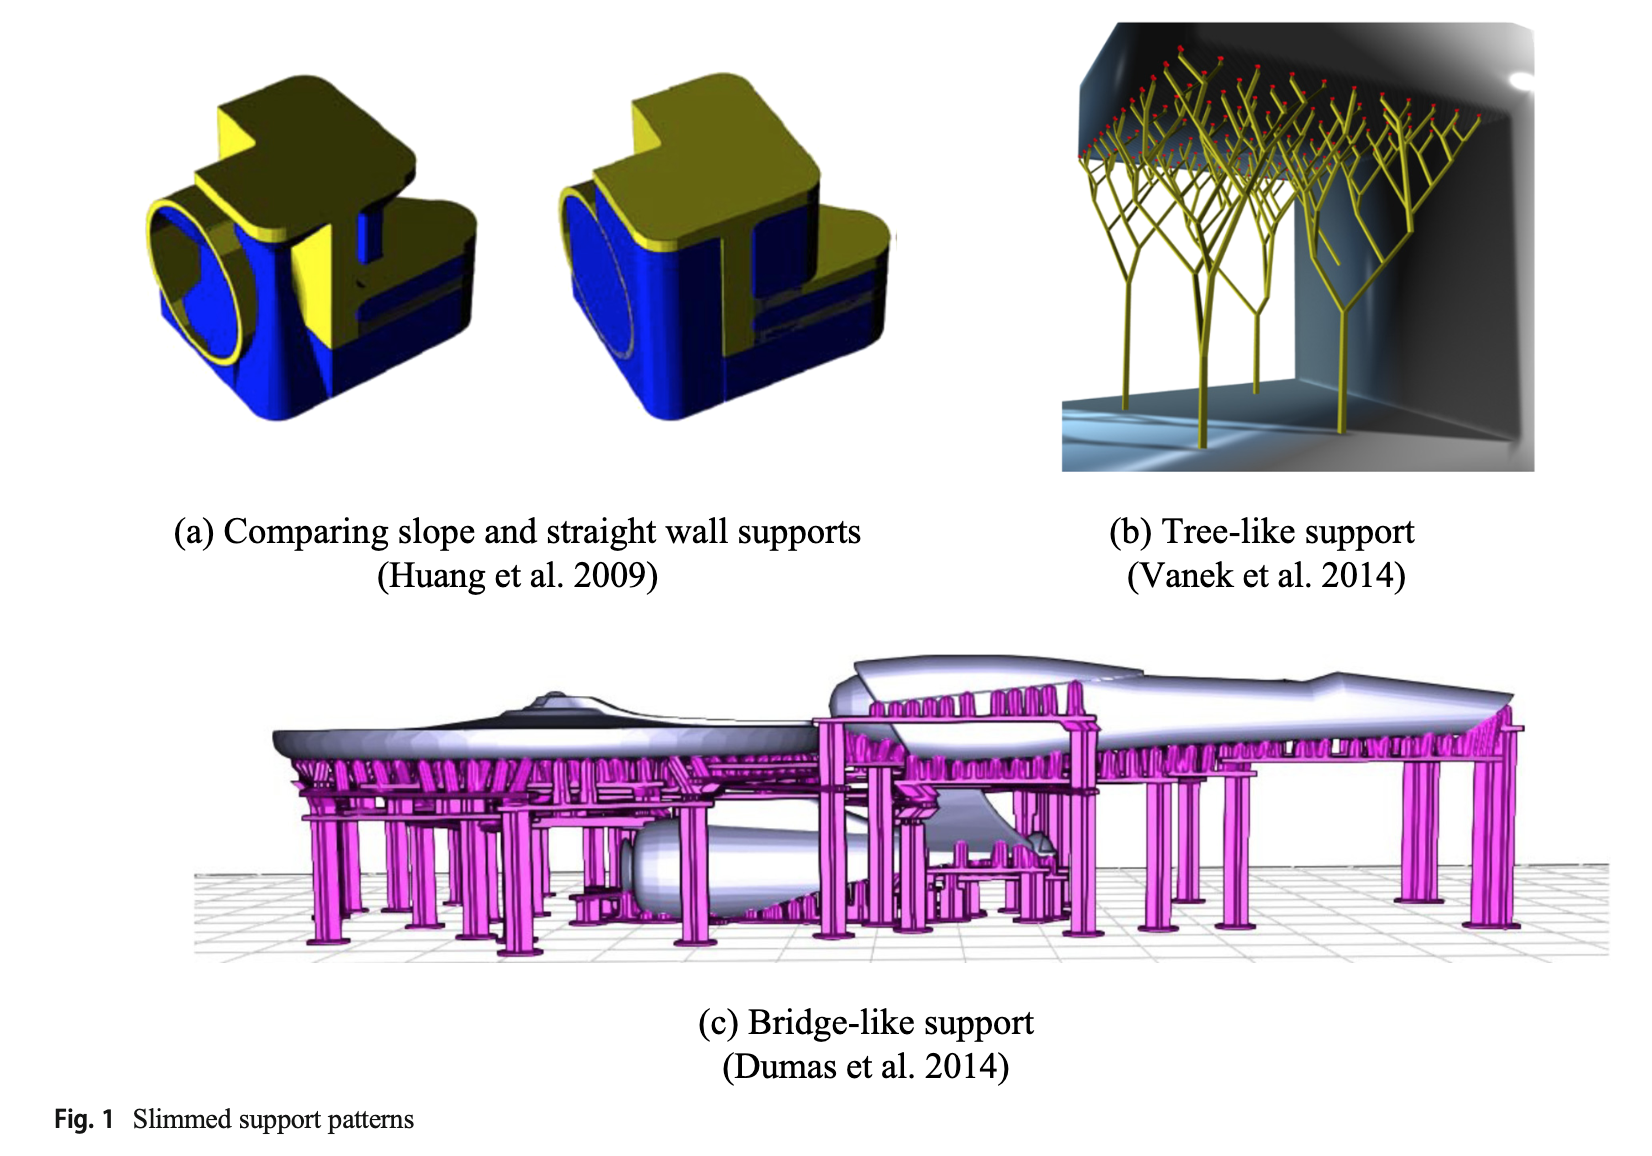
\includegraphics[width=5in]{Images/topopt1}
		\label{topopt1}
	\end{subfigure}
	%
	~
	\centering
	\begin{subfigure}[b]{1\textwidth}
		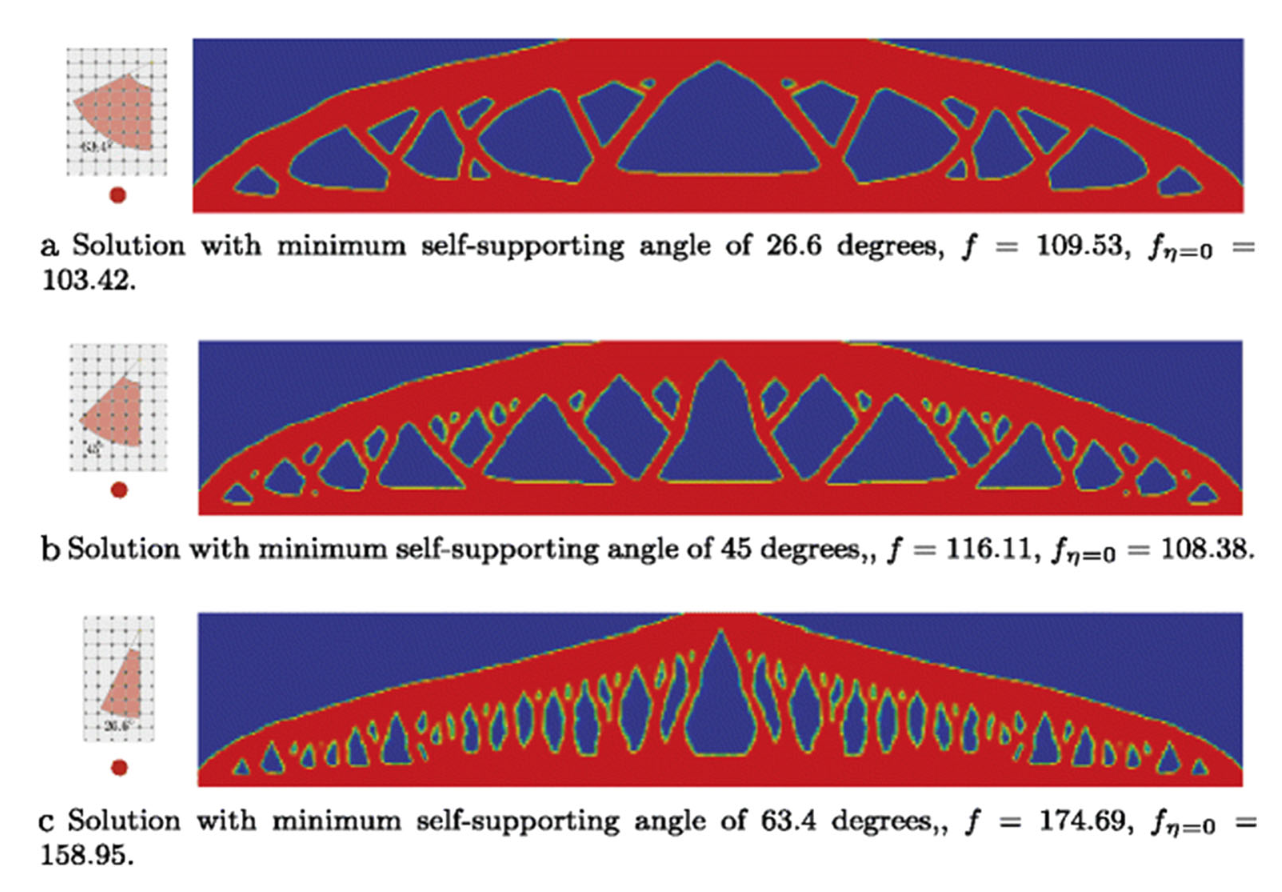
\includegraphics[width=3in]{Images/topopt2}
		\label{topopt2}
	\end{subfigure}
	\caption{Topology optimization algorithms to optimally design shapes and support structures for additively manufactured parts. While the major benefit of AM is in manufacturing unique, complex geometries the desired shapes sometimes require specific supports. a) Design of support structures for different slopes and shapes that may be difficult to print as-is. b) Topology optimization of a part to reduce the amount of sharp slopes which may cause print failure or residual stress build up. Images taken from the review on topology optimization in \cite{Liu2018}; images in b) taken from \cite{Huang2009, Vanek2014, Dumas2014}}
	\label{topopt}
\end{figure*}

Alloy design and experimental design focus around combinatorial screening of inputs to either search for \textit{new} properties or optimize on current properties. These optimizations reduce manufacturing cost, monetary or otherwise, and maximize performance capability. The same optimization can be applied to mechanical properties of parts. For structural materials, the goal is to optimize load bearing capacity or lifetime while minimizing the amount of material used. For aerospace, the goal is to minimize weight. Unique manufacturing geometries was one of the first intended applications of AM. Topology optimization (TO) focuses around exactly this task -- finding optimized topological structures for a given mechanical application. 

TO algorithms change the topology of a part by applying filters to different regions of its CAD model. A filter is a mathematical operation which reveals information about a region of pixels/voxels in a mesh. Filters are most often represented as a product of a filter matrix with a matrix of mesh pixel values. Topology optimization proceeds by generating a CAD model of an AM part and modeling its performance, such as testing performance under mechanical load through an FEA simulation. Filters are applied to the CAD mesh which selectively removes material from the part. Then, the mechanical performance of the new part is modeled, followed by further material removal. This process proceeds until either a minimum weight/volume condition is met or the mechanical performance of the part is degraded.

In additive, topology optimization serves an additional purpose: TO algorithms can find un-printable regions of a part. Unsupported structures, low angle slopes, and certain part orientations during building are prohibited in AM because they will cause part deformation. An unsupported slope at acute angles can lead to part deformation and warpage \cite{Gaynor2016}. Sacrificial support structures also need to be considered during topological optimization, along with the number of free-hanging features and the orientation of the part during manufacture. Several examples of parts with topology optimized support structures/geometries can be seen in Figure \ref{topopt}. Langelaar et al. developed an AM-specific TO algorithm which searches for regions of parts that have too little support for manufacture \cite{Langelaar2016, Langelaar2017}. Other additive specific algorithms have been designed for optimizing density of parts \cite{Zegard2016}. These algorithms augment the AM process, both by taking advantage of the ability to optimize unique geometries, and also by identifying regions of parts which are incompatible with AM.

